\documentclass[tikz,border=8pt]{standalone}

\begin{document}
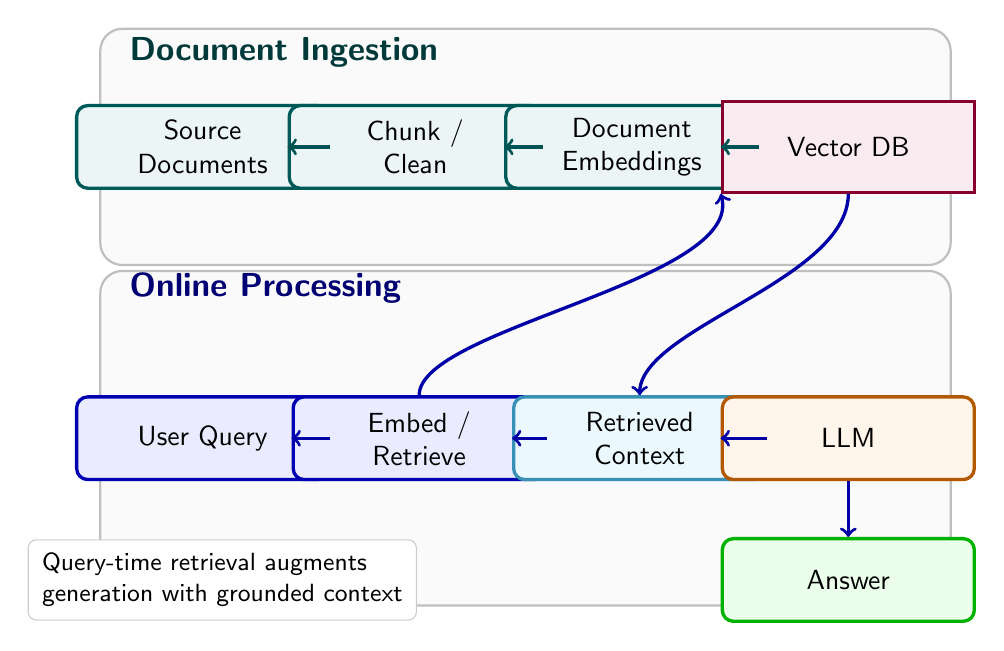
\begin{tikzpicture}[
  font=\sffamily,
  node distance=1.25cm,
  box/.style={
    draw=#1!70!black,
    fill=#1!8,
    rounded corners=4pt,
    very thick,
    minimum width=3.2cm,
    minimum height=1.05cm,
    align=center
  },
  store/.style={
    draw=#1!70!black,
    fill=#1!8,
    very thick,
    minimum width=3.2cm,
    minimum height=1.15cm,
    align=center
  },
  flow/.style={->, very thick, draw=black!70},
  dataflow/.style={->, very thick, draw=blue!65!black},
  ingestflow/.style={->, very thick, draw=teal!65!black},
  boundary/.style={
    draw=black!25,
    rounded corners=8pt,
    thick,
    fill=black!2
  }
]

\node[boundary, minimum width=10.8cm, minimum height=3.0cm] (ingestArea) at (0,2.35) {};
\node[anchor=west, font=\sffamily\bfseries\large, text=teal!45!black] at (-5.15,3.55) {Document Ingestion};

\node[boundary, minimum width=10.8cm, minimum height=4.25cm] (onlineArea) at (0,-1.35) {};
\node[anchor=west, font=\sffamily\bfseries\large, text=blue!45!black] at (-5.15,0.55) {Online Processing};

\node[box=teal] (docs) at (-4.1,2.35) {Source\\Documents};
\node[box=teal] (chunk) at (-1.4,2.35) {Chunk /\\Clean};
\node[box=teal] (docembed) at (1.35,2.35) {Document\\Embeddings};
\node[store=purple] (vectordb) at (4.1,2.35) {Vector DB};

\draw[ingestflow] (docs) -- (chunk);
\draw[ingestflow] (chunk) -- (docembed);
\draw[ingestflow] (docembed) -- (vectordb);

\node[box=blue] (query) at (-4.1,-1.35) {User Query};
\node[box=blue] (retrieve) at (-1.35,-1.35) {Embed /\\Retrieve};
\node[box=cyan] (context) at (1.45,-1.35) {Retrieved\\Context};
\node[box=orange] (llm) at (4.1,-1.35) {LLM};
\node[box=green] (answer) at (4.1,-3.15) {Answer};

\draw[dataflow] (query) -- (retrieve);
\draw[dataflow] (retrieve) -- (context);
\draw[dataflow] (context) -- (llm);
\draw[dataflow] (llm) -- (answer);

\draw[dataflow] (retrieve.north) .. controls (-1.35,0.05) and (2.8,0.65) .. (vectordb.south west);
\draw[dataflow] (vectordb.south) .. controls (4.1,0.65) and (1.45,0.05) .. (context.north);

\node[
  draw=black!20,
  fill=white,
  rounded corners=3pt,
  align=left,
  font=\sffamily\small,
  inner sep=5pt
] at (-3.85,-3.15) {
  Query-time retrieval augments\\
  generation with grounded context
};

\end{tikzpicture}
\end{document}
